%%%%%%%%%%%%%%%%%%%%%%%%%%%%%%%%%%%%%%%%%%%%%%%%%%%%%%%%%%%%%%%%%
% !TEX root = interimreport.tex
\clearpage
\chapter{NEW INSTRUCTIONS}\label{Ch9}
%%%%%%%%%%%%%%%%%%%%%%%%%%%%%%%%%%%%%%%%%%%%%%%%%%%%%%%%%%%%%%%%%

\section{SHLXOR Instruction}
We extended the instruction set by adding the SHLXOR instruction. The purpose of this instruction is to shift the first source operand one bit to the left and then XOR it with the second source operand. Then, the obtained result is stored in the destination register. By adding this instruction, we can perform this operation with a single instruction instead of using shift left and XOR instructions separately, making it more efficient.
Let’s give an example to make it clearer what this instruction does. RS1 and RS2 are source operands and RD is the output.
\\
RS1: 0x0101     RS2: 0xFFFF     RD: 0xFDFD
\\
0x0101 is shifted left by one and then XOR’ed with 0xFFFF, giving the result 0xFDFD.
As we mentioned, this new instruction requires two source registers and one destination register. Therefore, unlike the MLA instruction, we don’t need to create a new class to support it. There is already a class named ALU\_rr in the RISCVInstrinfo.td file that has two source and one destination register. Therefore, the new SHLXOR instruction is going to belong to the ALU\_rr class. The ALU\_rr class is given below.

\begin{lstlisting}
let hasSideEffects = 0, mayLoad = 0, mayStore = 0 in
class ALU_rr<bits<7> funct7, bits<3> funct3, string opcodestr,
bit Commutable = 0>
: RVInstR<funct7, funct3, OPC_OP, (outs GPR:\$rd), (ins GPR:\$rs1, GPR:\$rs2),
opcodestr, "\$rd, \$rs1, \$rs2"> {
let isCommutable = Commutable;
}
\end{lstlisting}

As we can see, encoding of this type of instructions consists of funct7, funct3, opcode, source registers, and the destination register. The encoding format and the other properties are described in the class. The source registers are described as inputs and the destination register is described as the output.
In the RISCVInstrInfoCrypt.td file, we add the definition of the SHLXOR instruction by using the ALU\_rr class. In this part, we define funct7, funct3, and the mnemonic of the new instruction as well as the schedulings.

\begin{lstlisting}
def SHLXOR : ALU_rr<0b0011000, 0b111, "shlxor">,
Sched<[WriteIALU, ReadIALU, ReadIALU]>;
\end{lstlisting}

Also in the same file, we define the instruction’s pattern. When we examine this definition, we can clearly see what the instruction performs and its pattern. In the inner parentheses, we can see the shifting of the first source operand by one bit. Then, the result of this shifting operation is used as an input for the XOR operation alongside the second source operand.

\begin{lstlisting}
def : Pat< (xor (shl GPR:\$src1, (i32 1)), GPR:\$src2),
(SHLXOR GPR:\$src1, GPR:\$src2)>;
\end{lstlisting}

After doing these, we can try it with a simple C code given below. 

\begin{lstlisting}[language=C++]
int a,b;

void shlxor() {
	a = 3;
	b = 5;
		
	a = b^(a<<1);
}
\end{lstlisting}

Let’s get an assembly output from this C code by running the following commands:

\begin{lstlisting}[language=Bash]
clang -S -target riscv32-linux-gnu -emit-llvm shlxor.c
<llvm-build-path>/build/bin/llc -mtriple=riscv32 shlxor.ll
\end{lstlisting}


%TODO lets set standard bin directory throughout thesis 
Here, CustomInstrLLVM is the folder that we built llvm in.

This C code basically shifts the variable a by one bit and XOR’s it with b variable. Then the result is stored in a. We can see that, the register that stores the value a is both the first source register and the destination register. The assembly output is given below.
%TODO find RISCV latex syntax 
%TODO and TableGen
\begin{lstlisting}%[language={[RISC-V]Assembler}]
shlxor:                                 # @shlxor
.Lfunc_begin0:
	.loc	0 4 0                           # shlx.c:4:0
	.cfi_sections .debug_frame
	.cfi_startproc
# %bb.0:
	addi	sp, sp, -16
	.cfi_def_cfa_offset 16
.Ltmp0:
	.loc	0 5 4 prologue_end              # shlx.c:5:4
	sw	ra, 12(sp)                      # 4-byte Folded Spill
	sw	s0, 8(sp)                       # 4-byte Folded Spill
	.cfi_offset ra, -4
	.cfi_offset s0, -8
	addi	s0, sp, 16
	.cfi_def_cfa s0, 0
	lui	a0, %hi(a)
	li	a1, 3
	sw	a1, %lo(a)(a0)
	.loc	0 6 4                           # shlx.c:6:4
	lui	a1, %hi(b)
	li	a2, 5
	sw	a2, %lo(b)(a1)
	.loc	0 9 6                           # shlx.c:9:6
	lw	a1, %lo(b)(a1)
	.loc	0 9 9 is_stmt 0                 # shlx.c:9:9
	lw	a2, %lo(a)(a0)
	.loc	0 9 7                           # shlx.c:9:7
	shlxor	a1, a2, a1
	.loc	0 9 4                           # shlx.c:9:4
	sw	a1, %lo(a)(a0)
	.loc	0 10 1 is_stmt 1                # shlx.c:10:1
	lw	ra, 12(sp)                      # 4-byte Folded Reload
	lw	s0, 8(sp)                       # 4-byte Folded Reload
	addi	sp, sp, 16
	ret
\end{lstlisting}

In the assembly output, we can see the SHLXOR instruction in line 29. a1 and a2 are the sources and a1 is also the destination as we can see.

In addition to that, we can check the DAG in order to see the effect of our newly added instruction. We can compare the DAGs before the new instruction is added and after. We can observe the DAG before SHLXOR is added in figure \ref{fig:shlxor_before}. In this DAG, shift left (shl) and xor instructions can be seen seperately

\begin{figure}[h!]
    \centering
    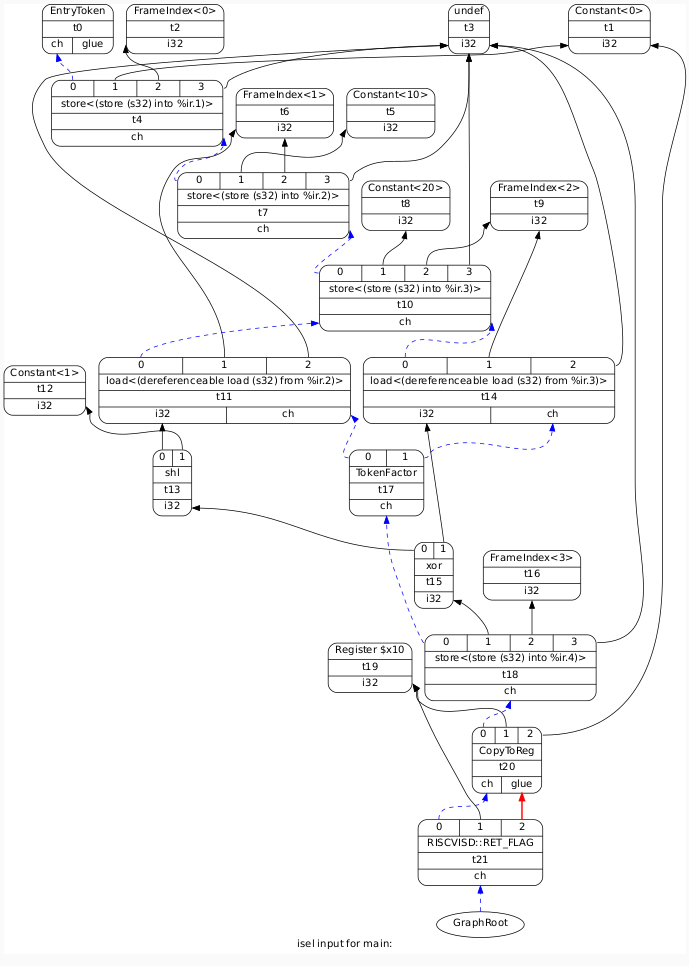
\includegraphics[scale= 0.3]{adding_new_instr/shlxor_before.png}
    \caption{DAG before SHLXOR is added}
    \label{fig:shlxor_before}
\end{figure}

The DAG after we add the SHLXOR instruction can be seen in figure \ref{fig:shlxor_after}. In this DAG, instead of two seperate instructions, a single SHLXOR instruction can be seen.

\begin{figure}[h!]
    \centering
    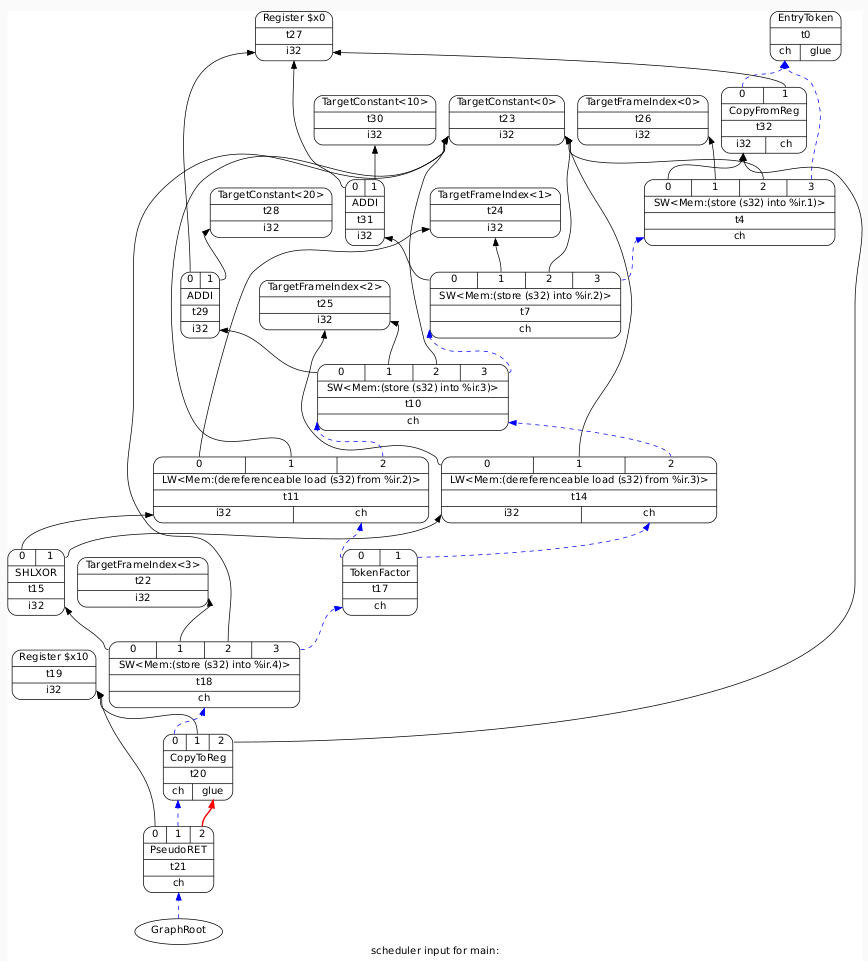
\includegraphics[scale= 0.3]{adding_new_instr/shlxor_after.png}
    \caption{DAG after SHLXOR is added}
    \label{fig:shlxor_after}
\end{figure}

\section{RORI Instruction}
One of the Instructions that we worked on is RORI instruction. The purpose of this instruction is to take the operand and rotate it to the right by the amount of the immediate value. This is different from shifting right using an immediate. When shifting a number to the right, the rightmost (least significant) bits are deleted and the leftmost (most significant) bits are filled in with zeros. On the other hand, when a number is rotated right, the least significant bits that are pushed out are not deleted but written into the most significant bits. We want to add add an instruction that performs this operation.

First of all, we tried pattern matching and added the definition and pattern of our new instruction to the InstrInfoCrypt.td file. However, that didn’t work and we couldn’t see the RORI instruction when we checked our assembly output created by using a simple C code that implements the rotation operation. This is because the pattern can have different combinations and may not match with what we expect. Therefore, the instruction cannot be recognized and we can’t see it in the assembly output.

Realizing that, we looked for other options and tried to make use of intrinsics and builtin functions. We added the definitions into the InstrInfoCrypt.td file.

\begin{lstlisting}
def ROTI : ALU_ri<0b101, "roti">;
\end{lstlisting}

It is ALU\_ri type because one of the operands is an immediate value and we only need one register for this instruction.

\begin{lstlisting}
def : Pat<(rotr GPR:\$rs1, simm12:\$imm12),
(ROTI GPR:\$rs1, simm12:\$imm12)>;
\end{lstlisting}

We used rotr here because we wanted to make use of the builtin function \_\_builtin\_rotateright32. rotr is defined in the RISVIselLowering.cpp file.

\begin{lstlisting}[language=C++]
if (Subtarget.hasStdExtZbb() || Subtarget.hasStdExtZbkb()) {
if (Subtarget.is64Bit())
setOperationAction({ISD::ROTL, ISD::ROTR}, MVT::i32, Custom);
} else {
setOperationAction({ISD::ROTL, ISD::ROTR}, XLenVT, Expand); 
}
\end{lstlisting}

However, we need to change the “Expand” to “Legal” in here otherwise we will not see the ROTI instruction in the assembly output.  This way, we are legalizing the action. If we don’t do this, we will see the fshr (funnel shift right) intrinsic in the .ll file but ROTI won’t make it into the assembly output. After doing these, we can try it with a simple C code. As mentioned before, we used a built in rotate function in the C code given below. 
%\ref{fig:c_code_with_builtin_function_for_roti}.

\begin{lstlisting}[language=C++]
int a;

void ROT() {
	a = 15;
	
	a = __builtin_rotateright32(a,2);	
}
\end{lstlisting}

This code rotates 15 to the right by 2 bits. We can obtain the .ll file by running the following command.

\begin{lstlisting}[language=Bash]
clang -S -target riscv32-linux-gnu -emit-llvm roti.c
\end{lstlisting}

The simplified contents of the .ll file is given below.

\begin{lstlisting}[language=llvm,style=nasm]

@a = dso_local global i32 0

define void @ROT() {
  store i32 15, i32* @a
  %1 = load i32, i32* @a
  %2 = call i32 @llvm.fshr.i32(i32 %1, i32 %1, i32 2)
  store i32 %2, i32* @a
  ret void
}
\end{lstlisting}

The fshr intrinsic is visible in the twelfth line. After that, the assembly output can be obtained by running the following command. 
%The assembly output is given in figure \ref{fig:roti_assembly_output}.

\begin{lstlisting}[language=Bash]
~/CustomInstrLLVM/build/bin/llc -mtriple=riscv32 roti.ll$
\end{lstlisting}

The obtained assembly output is given below.

\begin{lstlisting}
ROT:                                    # @ROT
.Lfunc_begin0:
	.loc	0 3 0                           # roti.c:3:0
	.cfi_sections .debug_frame
	.cfi_startproc
# \%bb.0:
	addi	sp, sp, -16
	.cfi_def_cfa_offset 16
.Ltmp0:
	.loc	0 4 4 prologue_end              # roti.c:4:4
	sw	ra, 12(sp)                      # 4-byte Folded Spill
	sw	s0, 8(sp)                       # 4-byte Folded Spill
	.cfi_offset ra, -4
	.cfi_offset s0, -8
	addi	s0, sp, 16
	.cfi_def_cfa s0, 0
	lui	a0, \%hi(a)
	li	a1, 15
	sw	a1, \%lo(a)(a0)
	.loc	0 11 30                         # roti.c:11:30
	lw	a1, \%lo(a)(a0)
	.loc	0 11 6 is_stmt 0                # roti.c:11:6
	roti	a1, a1, 2
	.loc	0 11 4                          # roti.c:11:4
	sw	a1, \%lo(a)(a0)
	.loc	0 14 1 is_stmt 1                # roti.c:14:1
	lw	ra, 12(sp)                      # 4-byte Folded Reload
	lw	s0, 8(sp)                       # 4-byte Folded Reload
	addi	sp, sp, 16
	ret
\end{lstlisting}

The ROTI instruction can be seen in the assembly output in line 23. As expected, it uses one register as both  the destination and the source alongside an immediate value.

This way, we succesfully obtained the ROTI instruction. However, using the builtin function while writing the C code wasn’t the prettiest solution. Therefore, we looked further into how we can implement this. After that, we realized that there is a bit manipulation extension for RISCV and what we need was in the RISCVInstrInfoZb.td file. This file contains the instruction extensions for bit manipulations. These instructions operate on the bits of the data and RORI is one of those instructions. However, in order to utilize this extension, we need to add some flags to the command while running clang in order to get an assembly output from the C code we write. The simple C code for RORI is given below .%in figure \ref{fig:c_code_for_rori}.

\begin{lstlisting}[language=C++]
#define XLEN 32
#include <stdint.h>
#define uint_xlen_t uint32_t

uint_xlen_t rotimm(uint_xlen_t rs1)
{
uint_xlen_t a = 0;
a = ((rs1>>2) | (rs1<<(XLEN-2)));
return a;
}
\end{lstlisting}

Here, we use 32 as the length because our target is 32-bit and the rotation is implemented in the eighth line. After that, we run the following command with additional flags as mentioned before.

\begin{lstlisting}[language=Bash]
clang --target=riscv32 -O -S rori.c -march=rv32imaczbb
\end{lstlisting}

Here, -O defines the level of optimization. -S is used for getting an assembly file as an output. rori.c is the name of our simple C code. -march=rv32imaczbb designates that we want to utilize the zbb subgroup of the bit manipulation extension. The assembly output is given below.%in figure \ref{fig:rori_assembly_output}.

\begin{lstlisting}
	.text
	.attribute	4, 16
	.attribute	5, "rv32i2p0_m2p0_a2p0_c2p0_zbb1p0"
	.file	"rori.c"
	.globl	rotimm
	.p2align	1
	.type	rotimm,@function
rotimm:
	rori	a0, a0, 2
	ret
.Lfunc_end0:
	.size	rotimm, .Lfunc_end0-rotimm

	.ident	"Ubuntu clang version 14.0.0-1ubuntu1"
	.section	".note.GNU-stack","",@progbits
	.addrsig
\end{lstlisting}

This way, we managed to succesfully obtain RORI instruction in the assembly output.

\section{NAXOR Instruction}

S-box algorithm includes a certain pattern that is used repeatedly. Not and xor pattern is used five times in an s-box cycle. This pattern is lowered into one instruction using TableGen. Definition and specifications of the pattern are added to RISCVInstrInfoCrypt.td file. After matching this pattern 15 rows of the assembly file is reduced to one single instruction. For future works in this field, this pattern can be implemented in a single cycle by adding a new extension to the Ibex core.  

\begin{lstlisting}
def NAXOR : ALU_rrr<0b11, 0b100, "naxor">,
Sched<[WriteIMul, ReadIMul, ReadIMul]>;
\end{lstlisting}

Since there are three variables in this instruction, custom ALU\_rrr class is used which is explained in code \ref{lst:ALU_rrr}. 11 and 100 numbers are used for funct2 and funct3.
\\\\
\begin{lstlisting}
def : Pat< (xor (and (not GPR:$src1), GPR:$src2), GPR:$src3),
(NAXOR GPR:$src1, GPR:$src2, GPR:$src3)>;
\end{lstlisting}

This pattern is used 5 times in the rectangular shape of the \ref{fig:bit_manipulation_extension_groupings}. NAXOR instruction reduces 15 instructions into 5 instructions.
\\\\
\begin{figure}
    \centering
    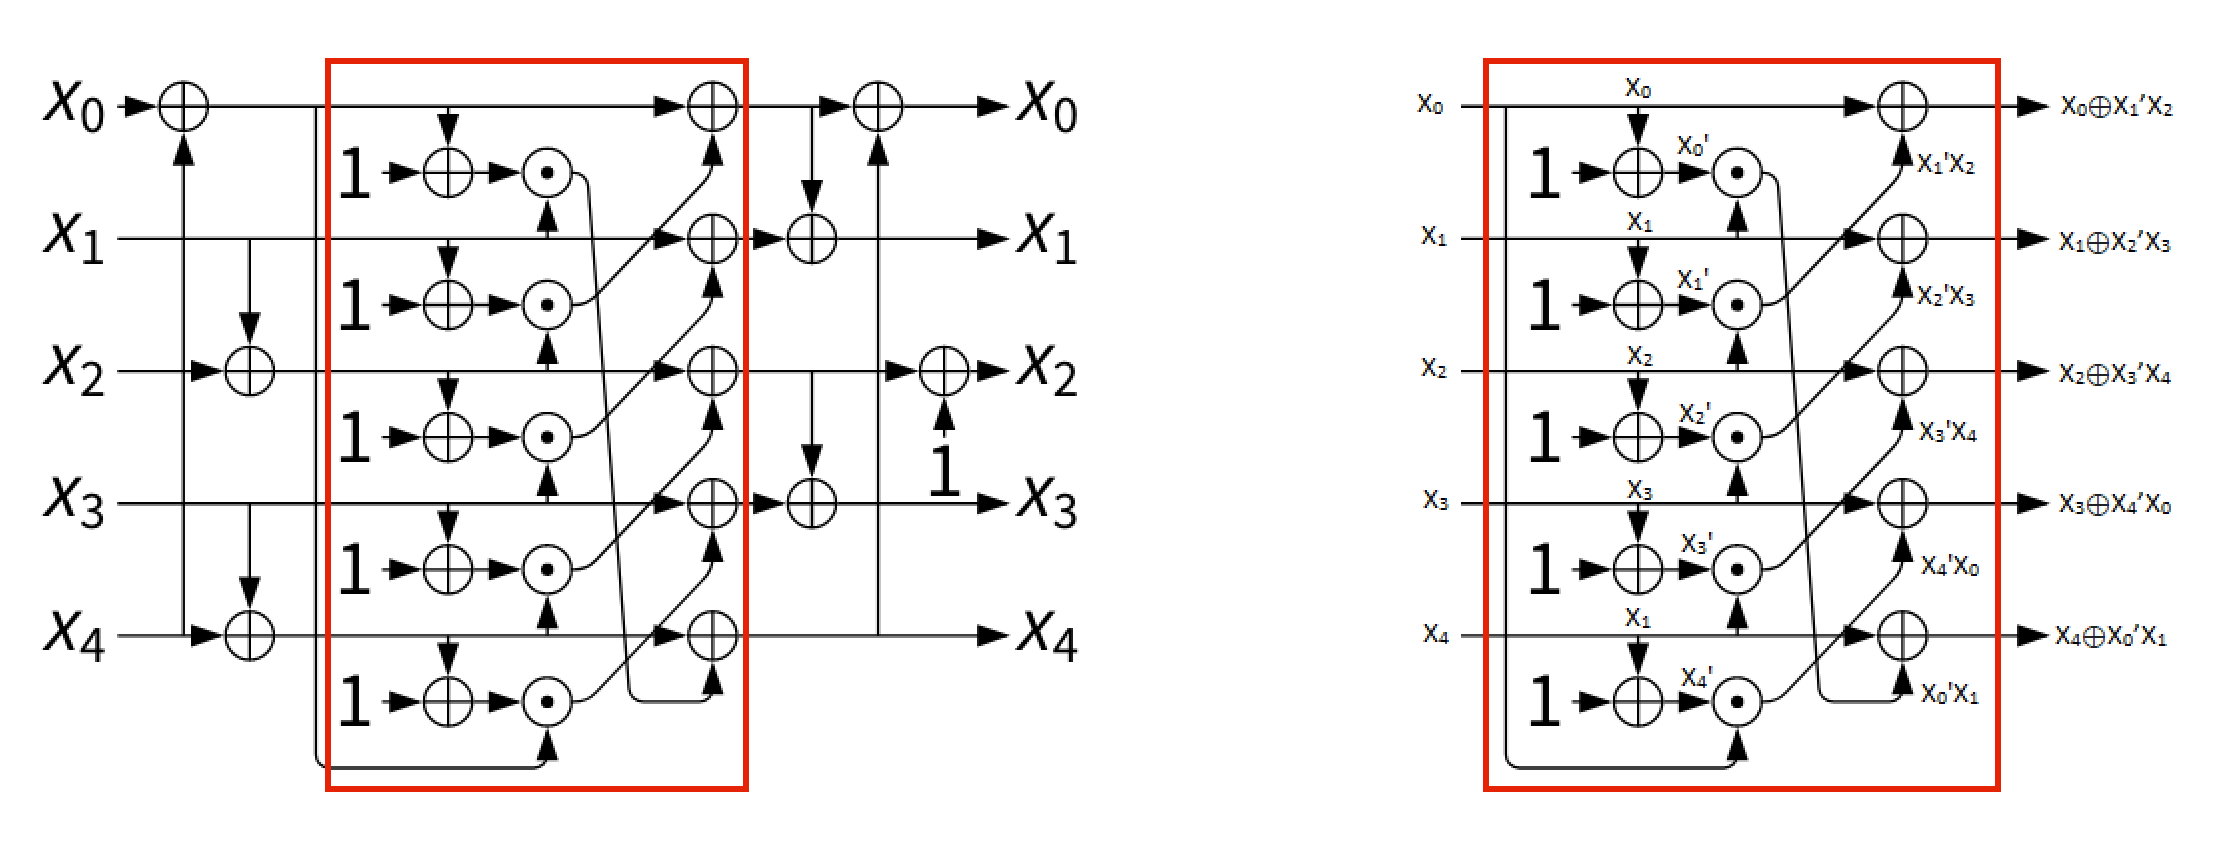
\includegraphics[scale=0.3]{adding_new_instr/sbox_naxor_pattern.png}
    \caption{NAXOR patterns in s-box algorithm}
    \label{fig:sbox_naxor_pattern}
\end{figure}

\begin{figure}
    \centering
    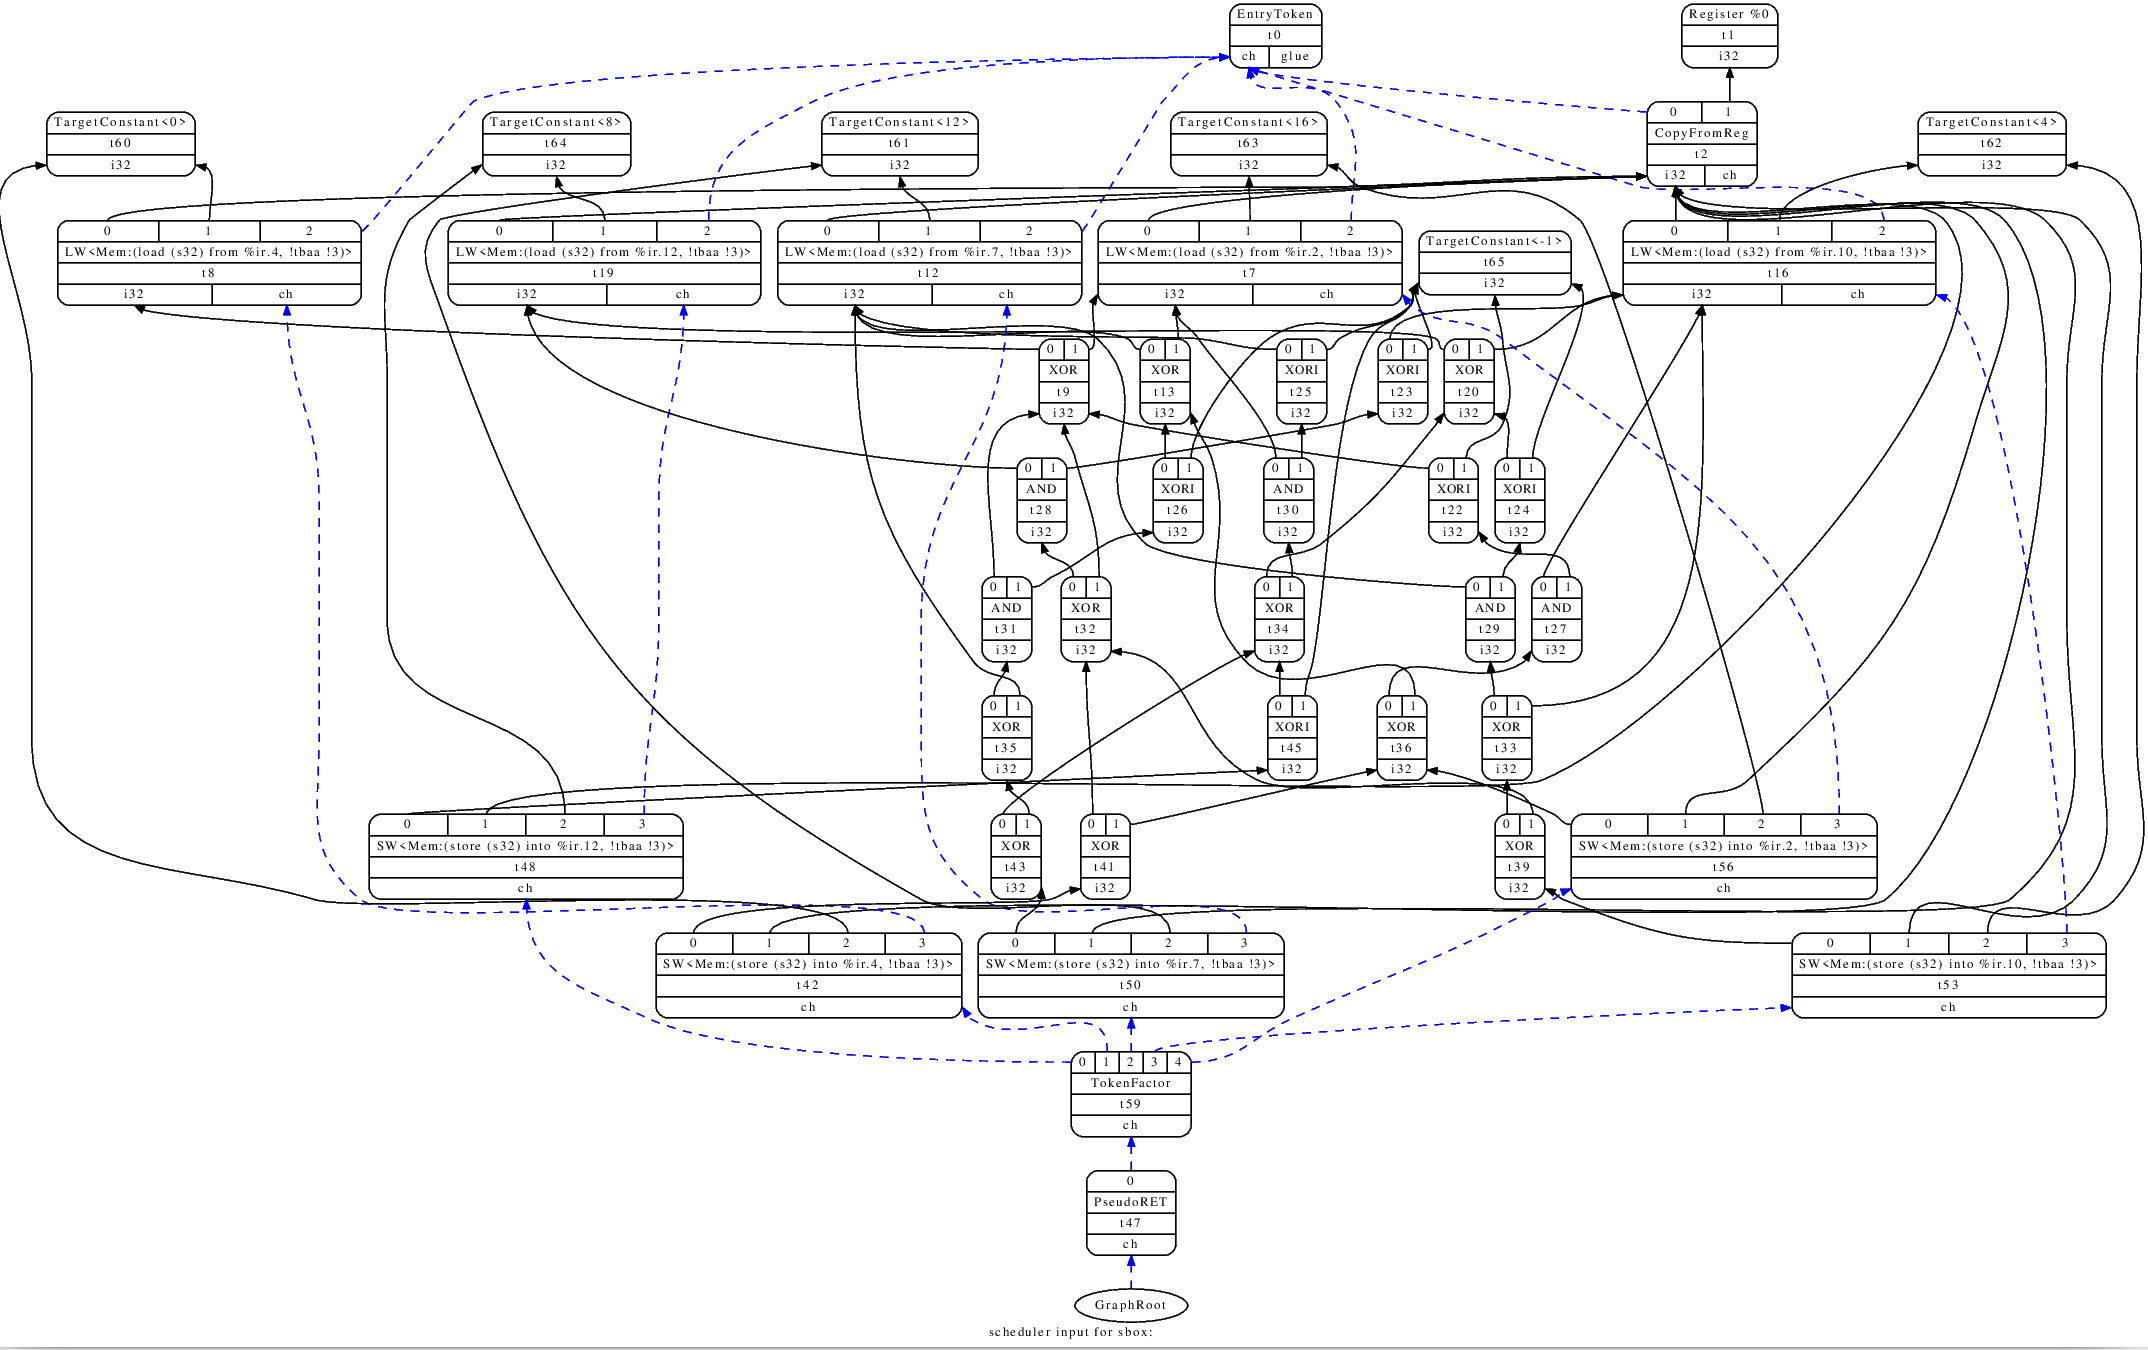
\includegraphics[scale=0.2]{adding_new_instr/naxor_sched.png}
    \caption{Dag diagram output for the s-box algorithm before scheduling}
    \label{fig:naxor_sched_diagram}
\end{figure}

\begin{figure}
    \centering
    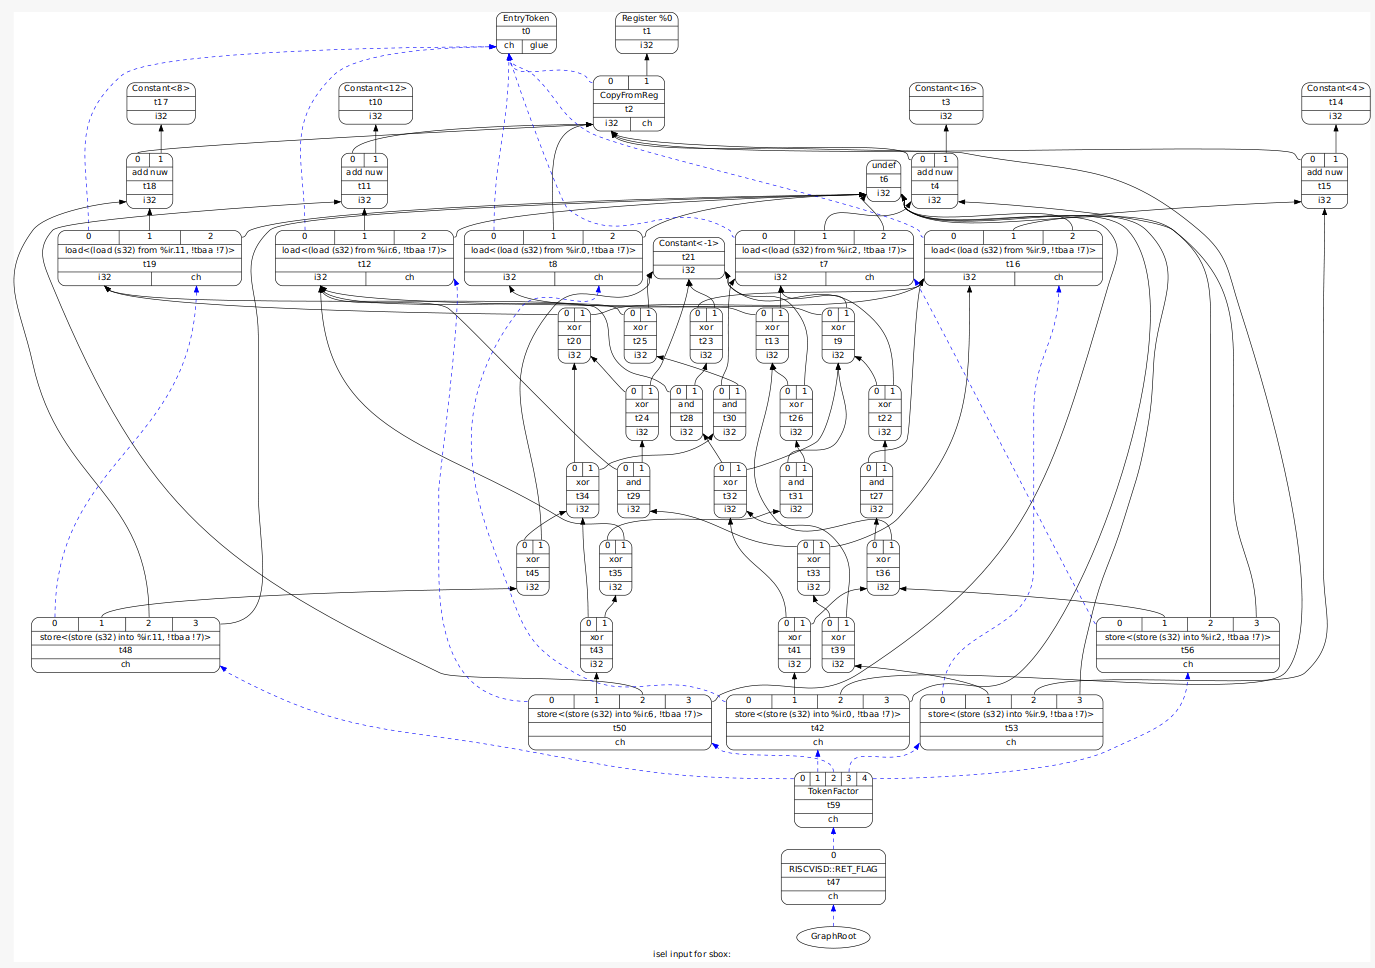
\includegraphics[scale=0.35]{adding_new_instr/naxor_dag_diagram.png}
    \caption{Dag diagram output for the s-box algorithm}
    \label{fig:naxor_dag_diagram}
\end{figure}

\begin{lstlisting}[caption= C code input for the S-box algorithm]

	typedef struct {
  int x[5];
} ascon_state_t;

void sbox(ascon_state_t state) {
int t0, t1, t2, t3, t4;
state.x[0] ^= state.x[4];
state.x[4] ^= state.x[3];
state.x[2] ^= state.x[1];
t0  = state.x[0];
t1  = state.x[1];
t2  = state.x[2];
t3  = state.x[3];
t4  = state.x[4];
t0 =~ t0;    
t1 =~ t1;    
t2 =~ t2;    
t3 =~ t3;    
t4 =~ t4;
t0 &= state.x[1];
t1 &= state.x[2];
t2 &= state.x[3];
t3 &= state.x[4];
t4 &= state.x[0];
state.x[0] ^= t1;
state.x[1] ^= t2;
state.x[2] ^= t3;
state.x[3] ^= t4;
state.x[4] ^= t0;
state.x[1] ^= state.x[0];
state.x[0] ^= state.x[4];
state.x[3] ^= state.x[2];
state.x[2] =~ state.x[2];

return;
}

\end{lstlisting}

\begin{minipage}{0.95\linewidth}

\lstinputlisting[caption={Optimized S-box LLVM IR}, language=llvm, style=nasm]{../s-box/keccakO3.ll}

\end{minipage}

%\\\\
\begin{lstlisting}[caption= Assembly output without NAXOR instruction]
    .text
	.attribute	4, 16
	.attribute	5, "rv32i2p0"
	.file	"s-box.c"
	.globl	sbox                            # -- Begin function sbox
	.p2align	1
	.type	sbox,@function
sbox:                                   # @sbox
	.cfi_startproc
# \%bb.0:
	lw	a1, 16(a0)
	lw	a2, 0(a0)
	lw	a3, 12(a0)
	lw	a4, 4(a0)
	lw	a5, 8(a0)
	xor	a2, a2, a1
	xor	a6, a3, a1
	xor	a7, a5, a4
	not	t0, a2
	not	t1, a4
	not	t2, a7
	not	t3, a3
	not	t4, a6
	and	t0, a4, t0
	and	a5, a5, t1
	and	t1, a3, t2
	and	a1, a1, t3
	and	t2, a2, t4
	xor	a2, a2, a5
	xor	a4, t1, a4
	xor	a1, a7, a1
	xor	a3, t2, a3
	xor	a5, t0, a6
	sw	a5, 16(a0)
	xor	a4, a4, a2
	sw	a4, 4(a0)
	xor	a2, a2, a5
	sw	a2, 0(a0)
	xor	a3, a3, a1
	sw	a3, 12(a0)
	not	a1, a1
	sw	a1, 8(a0)
	ret
.Lfunc_end0:
	.size	sbox, .Lfunc_end0-sbox
	.cfi_endproc
                                        # -- End function
	.ident	"clang version 17.0.0 (https://github.com/llvm/llvm-project.git e3dd9f7e66fec22986605da2dcd8120a7864455d)"
	.section	".note.GNU-stack","",@progbits

\end{lstlisting}


\begin{figure}
    \centering
    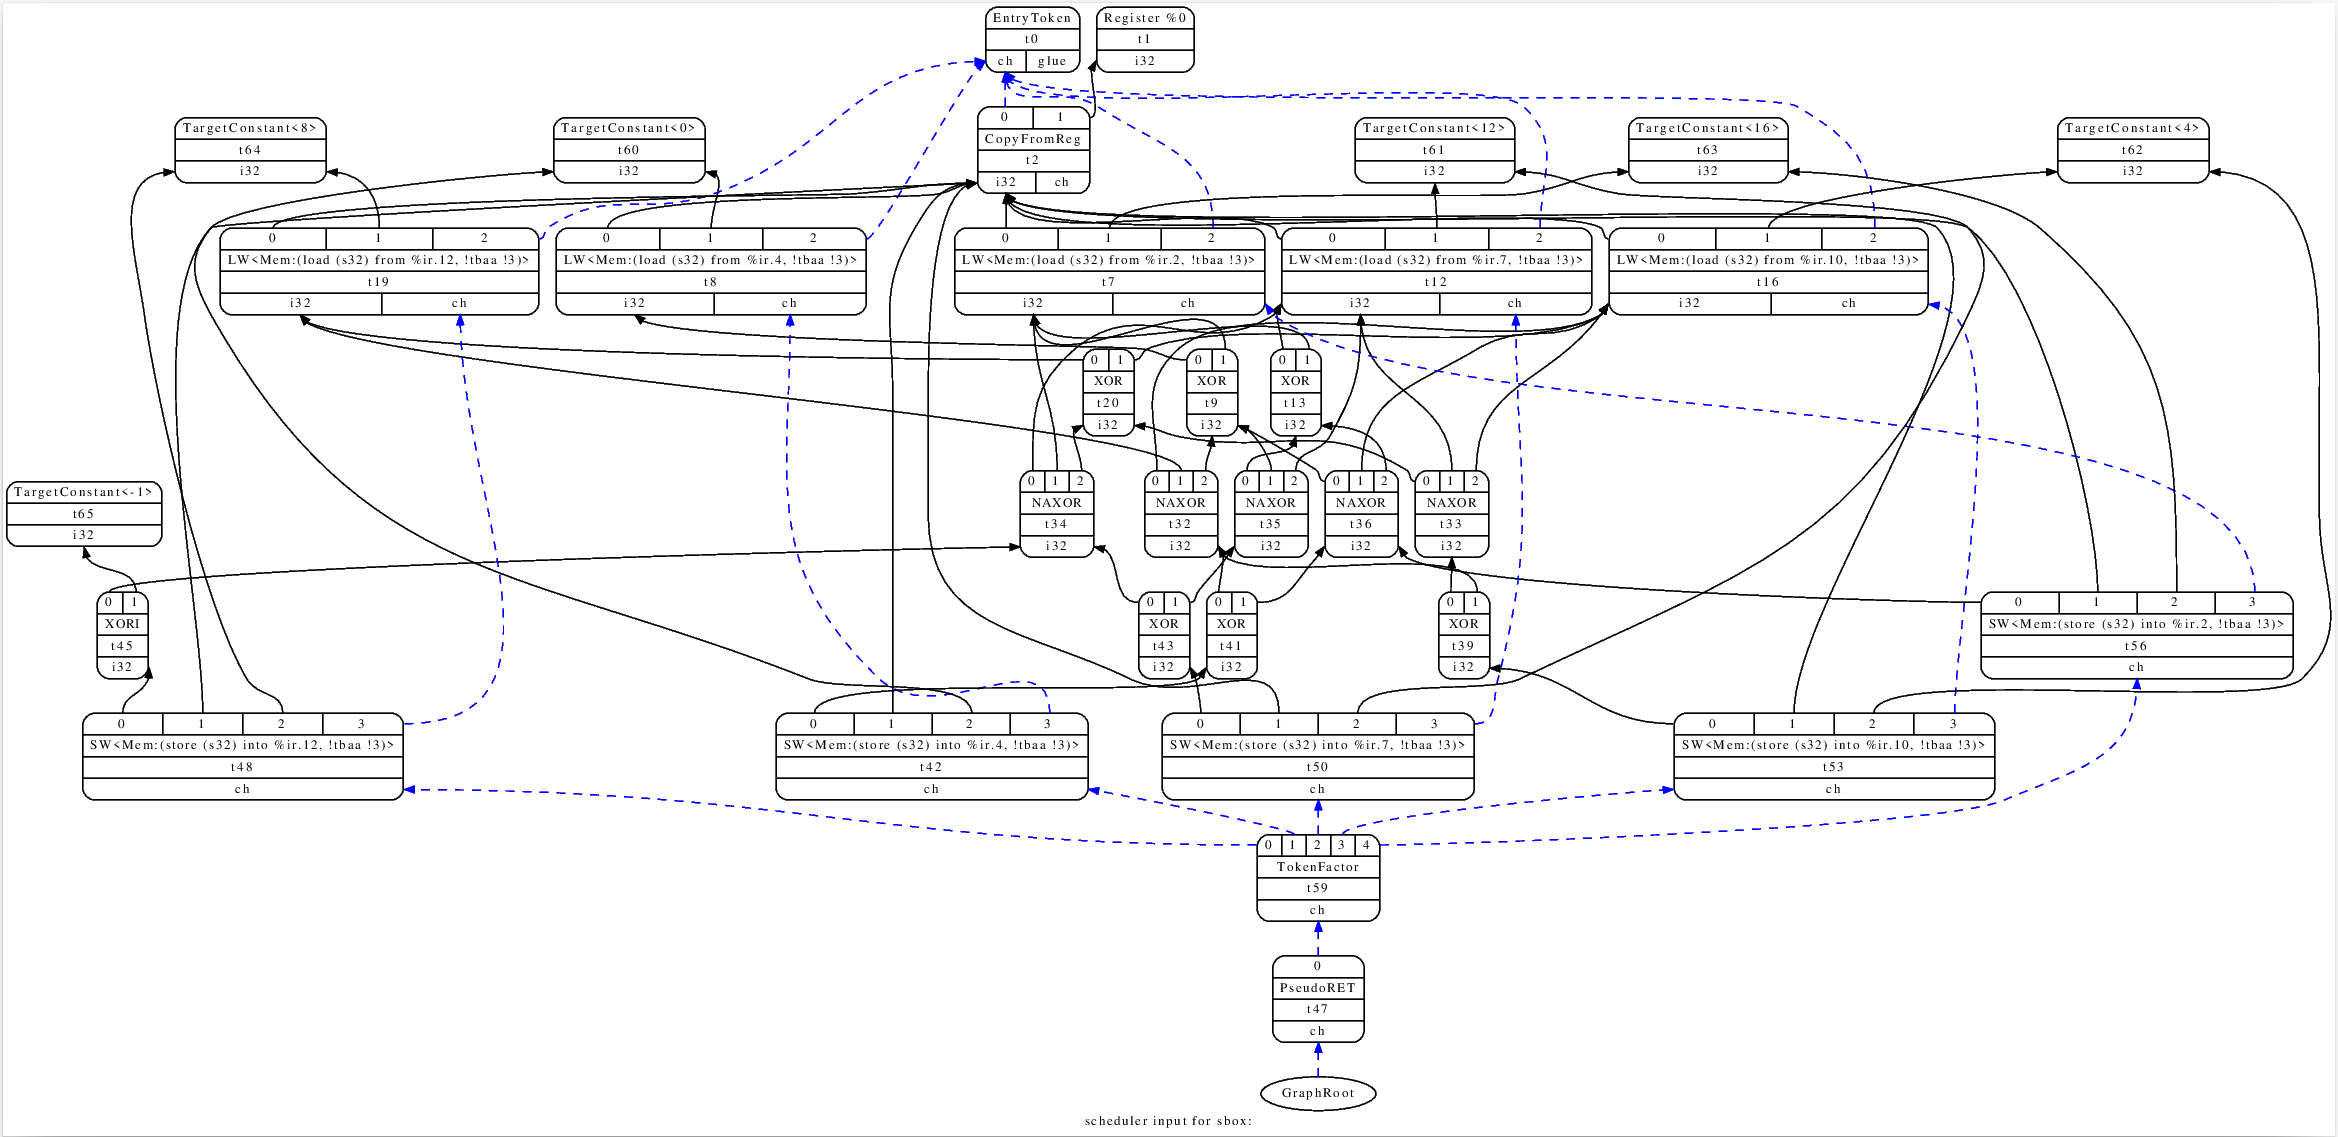
\includegraphics[scale=0.19]{adding_new_instr/naxor_match.png}
    \caption{Dag diagram output for the s-box algorithm after NAXOR instruction is matched}
    \label{fig:naxor_match_diagram}
\end{figure}


\begin{lstlisting}[caption= Assembly output with NAXOR instruction]
    .text
	.attribute	4, 16
	.attribute	5, "rv32i2p0"
	.file	"s-box.c"
	.globl	sbox                            # -- Begin function sbox
	.p2align	1
	.type	sbox,@function
sbox:                                   # @sbox
	.cfi_startproc
# \%bb.0:
	lw	a1, 16(a0)
	lw	a2, 0(a0)
	lw	a3, 12(a0)
	lw	a4, 4(a0)
	lw	a5, 8(a0)
	xor	a2, a2, a1
	xor	a6, a3, a1
	xor	a7, a5, a4
	naxor	a5, a4, a5 ,a2
	naxor	t0, a7, a3 ,a4
	naxor	a1, a3, a1 ,a7
	naxor	a3, a6, a2 ,a3
	naxor	a2, a2, a4 ,a6
	sw	a2, 16(a0)
	xor	a4, t0, a5
	sw	a4, 4(a0)
	xor	a2, a2, a5
	sw	a2, 0(a0)
	xor	a3, a3, a1
	sw	a3, 12(a0)
	not	a1, a1
	sw	a1, 8(a0)
	ret
.Lfunc_end0:
	.size	sbox, .Lfunc_end0-sbox
	.cfi_endproc
                                        # -- End function
	.ident	"clang version 17.0.0 (https://github.com/llvm/llvm-project.git e3dd9f7e66fec22986605da2dcd8120a7864455d)"
	.section	".note.GNU-stack","",@progbits

\end{lstlisting}

15 lines of not, and, xor operations are reduced to 5 NAXOR instructions.
\\\\






\section{LXR Instruction}

S-box algorithm uses multiple inputs and outputs and they are supposed to be loaded and stored to the registers during implementation. An example pattern is matched using TableGen. LXR instruction covers an xor operation of two loaded numbers. ALU\_rrr class (\ref{lst:ALU_rrr}) is used to match the pattern since three registers are used in the instruction.

\begin{lstlisting}
let mayLoad = 1 in{
def LXR : ALU_rr<0b0011011, 0b101, "lxr">,
Sched<[WriteIALU, ReadIALU, ReadIALU]>;
}
\end{lstlisting}

ALU\_rr class is used and 0011011, 101 numbers are used for opcodes. mayLoad flag is 1 to enable the load instruction in pattern.
\\
\begin{lstlisting}
def : Pat< (xor (load GPR:$rs1),(load GPR:$rs2)),
(LXR GPR:$rs1,GPR:$rs2)>;
\end{lstlisting}

LXR instruction covers the xor operation of two loaded numbers.
\\

\begin{figure}
    \centering
    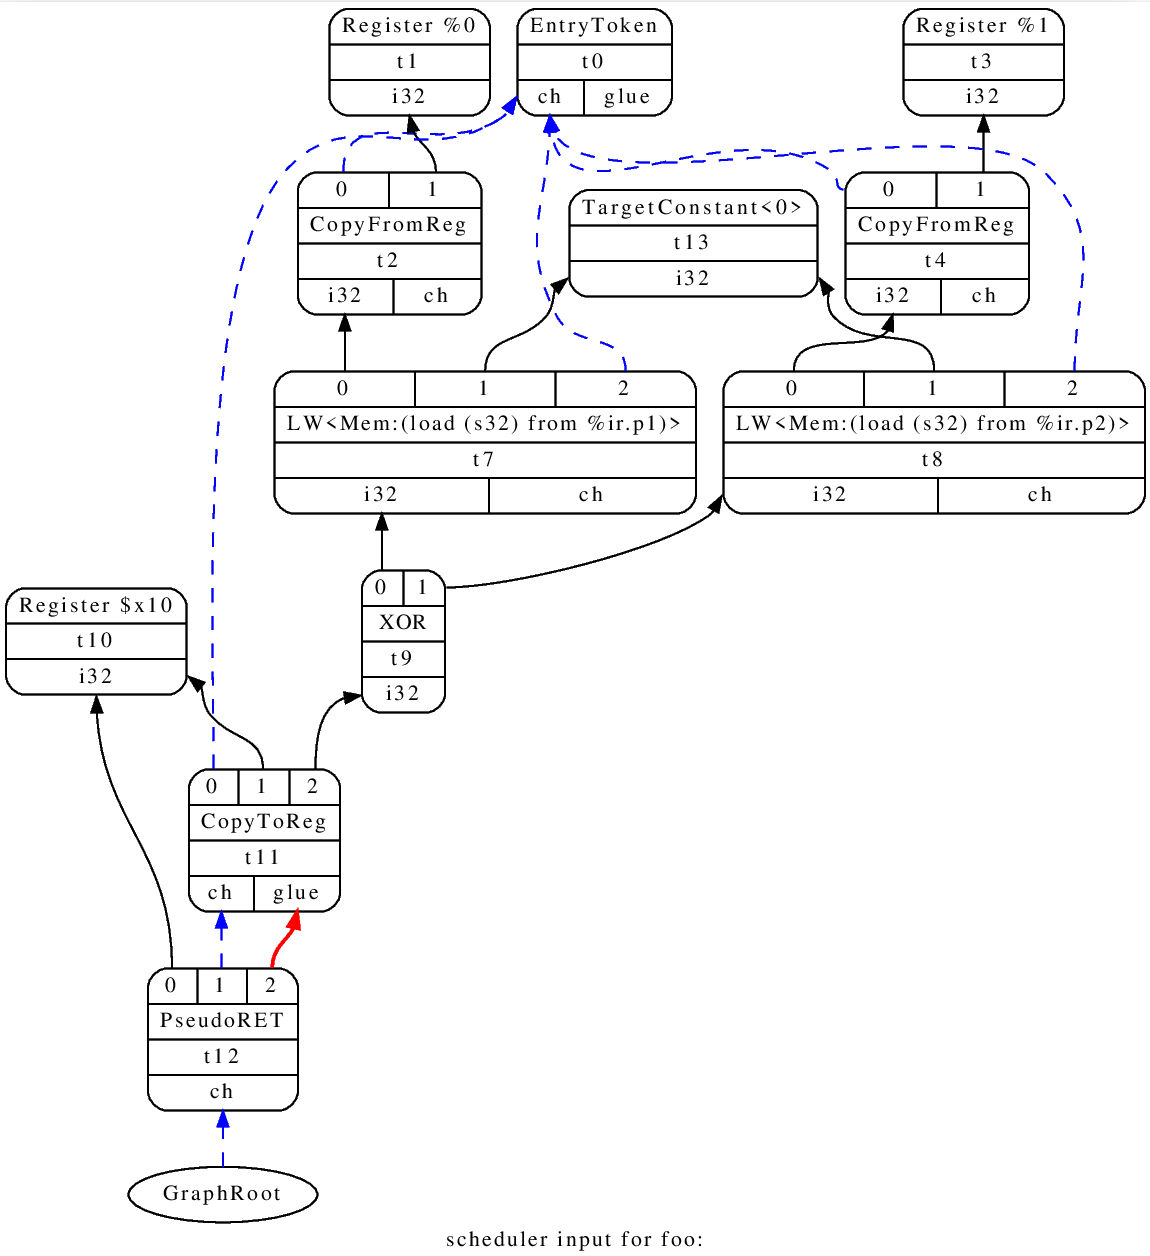
\includegraphics[scale=0.3]{adding_new_instr/lxr_sched.png}
    \caption{Dag diagram for the example LXR algorithm before scheduling}
    \label{fig:lxr_sched_diagram}
\end{figure}


\begin{figure}
    \centering
    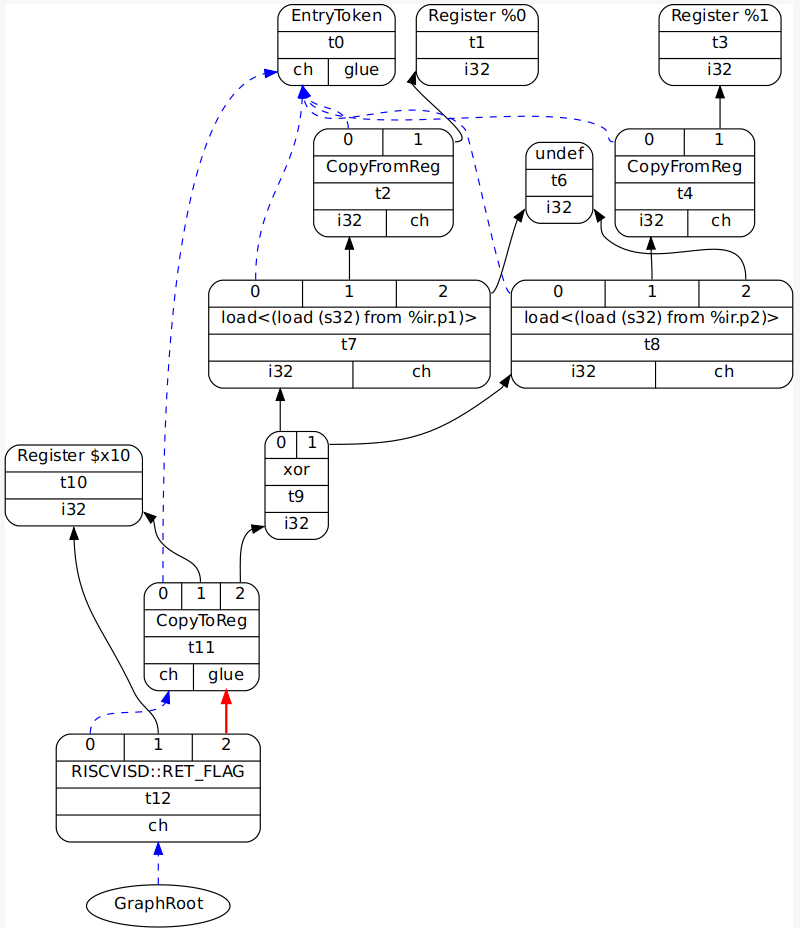
\includegraphics[scale=0.5]{adding_new_instr/lxr_dag_diagram.png}
    \caption{Dag diagram output for the example LXR algorithm}
    \label{fig:lxr_dag_diagram}
\end{figure}

\begin{lstlisting}[caption={Intermediate Representation code input for LXR algorithm}, language=llvm, style=nasm]
    define i32 @foo(ptr %p1, ptr %p2) {
        %a = load i32, ptr %p1
        %b = load i32, ptr %p2
        %res = xor i32 %a, %b
        ret i32 %res
      }
\end{lstlisting}


%\\\\

\begin{lstlisting}[caption= Assembly output without LXR instruction]
      
          .text
          .attribute	4, 16
          .attribute	5, "rv32i2p0"
          .file	"lxr.ll"
          .globl	foo                             # -- Begin function foo
          .p2align	2
          .type	foo,@function
      foo:                                    # @foo
          .cfi_startproc
      # \%bb.0:
          lw	a0, 0(a0)
          lw	a1, 0(a1)
          xor	a0, a0, a1
          ret
      .Lfunc_end0:
          .size	foo, .Lfunc_end0-foo
          .cfi_endproc
                                              # -- End function
          .section	".note.GNU-stack","",@progbits
      
      
\end{lstlisting}


\begin{figure}
    \centering
    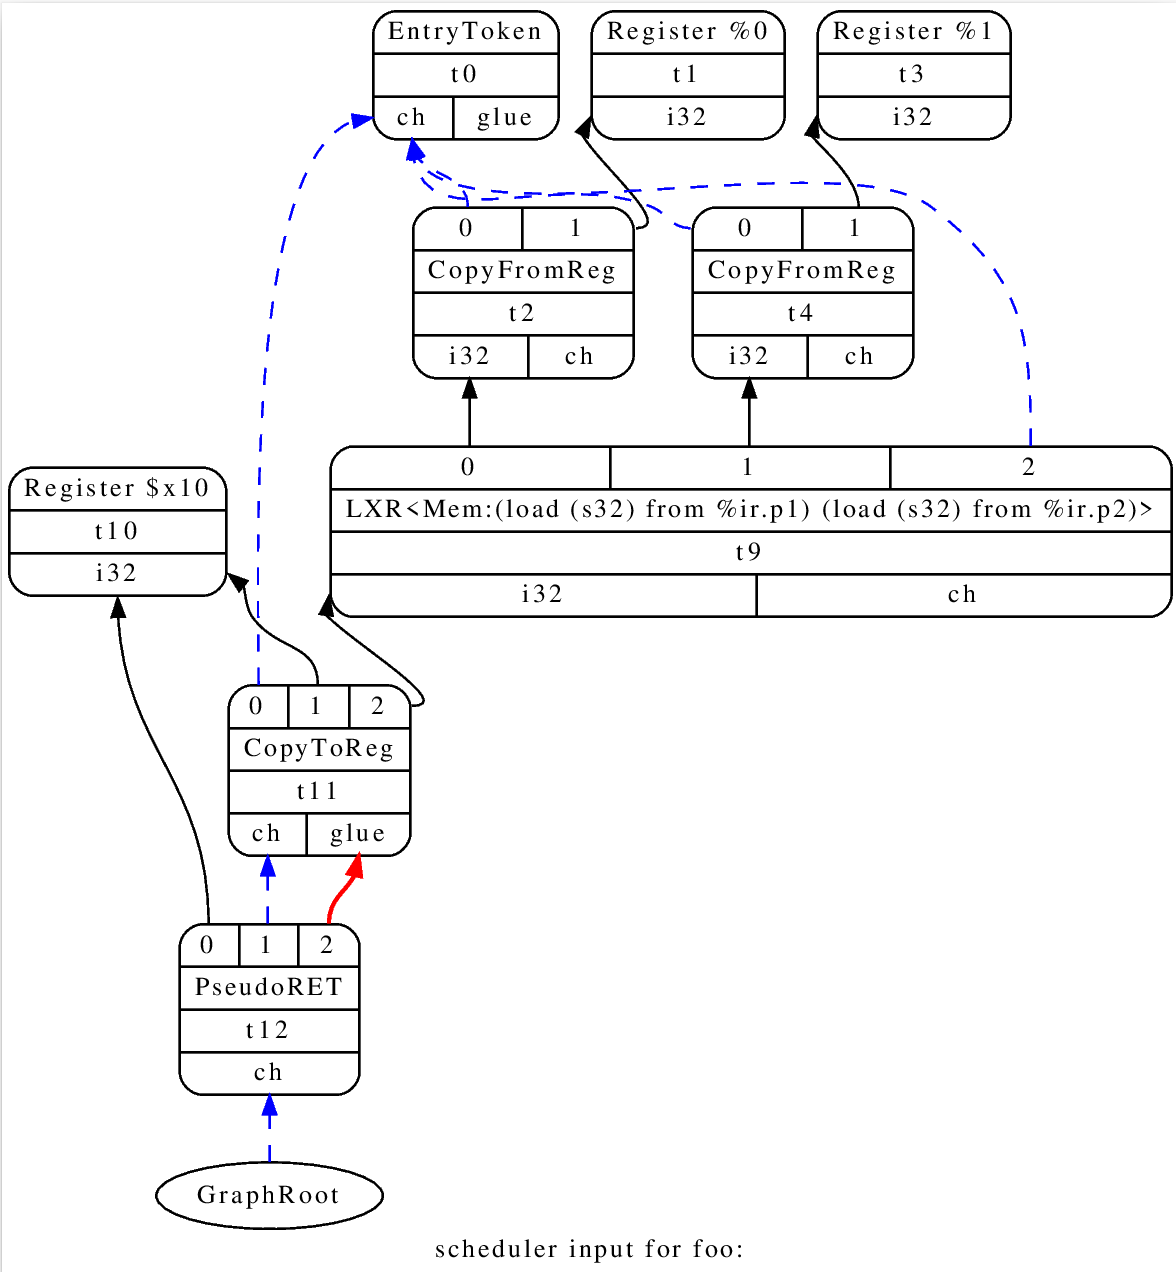
\includegraphics[scale=0.3]{adding_new_instr/lxr_match.png}
    \caption{Dag diagram output for the example LXR algorithm after LXR instruction is matched}
    \label{fig:lxr_match}
\end{figure}


\begin{lstlisting}[caption= Assembly output with LXR instruction]
    .text
	.attribute	4, 16
	.attribute	5, "rv32i2p0"
	.file	"lxr.ll"
	.globl	foo                             # -- Begin function foo
	.p2align	2
	.type	foo,@function
foo:                                    # @foo
	.cfi_startproc
# \%bb.0:
	lxr	a0, a0, a1
	ret
.Lfunc_end0:
	.size	foo, .Lfunc_end0-foo
	.cfi_endproc
                                        # -- End function
	.section	".note.GNU-stack","",@progbits
\end{lstlisting}

Two loads and one xor instructions are reduced to LXR instruction.
\\\\
